\documentclass[preview,border=5pt]{standalone}
\usepackage{teaching}
\begin{document}

\centering

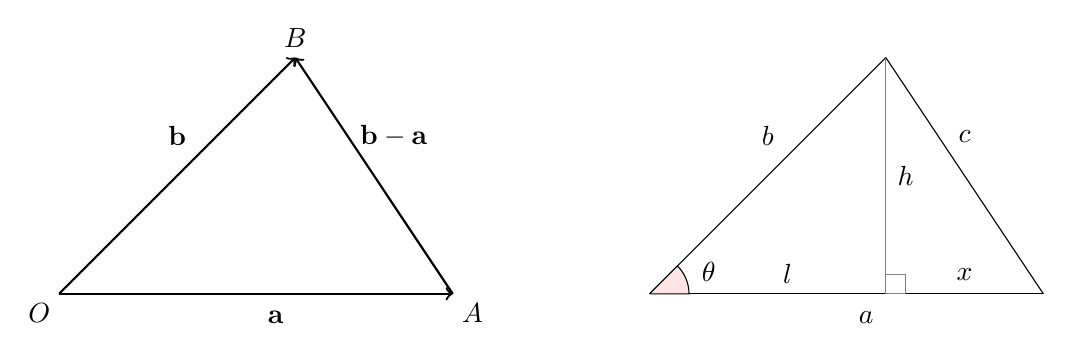
\begin{tikzpicture}[scale=5, inner sep=0.1mm]

\draw[thick,->] (0,0) -- (1,0);
\draw[thick,->] (0,0) -- (0.6,0.6);
\draw[thick,->] (1,0) -- (0.6,0.6);
%\draw[black!50!white] (0.6,0.6) -- (0.6,0);
%\draw[black!50!white] (0.6,0) -- (0.65,0) -- (0.65,0.05) -- (0.6,0.05);
%\draw[fill=red!10!white] (0,0) -- (0.1,0) arc (0:45:0.1cm)  -- (0,0);
\node at (0.55,-0.06) {$\mathbf{a}$};
%\node at (0.8,0.05) {$x$};
%\node at (0.35,0.05) {$l$};
%\node at (0.15,0.055) {$\psi$};
%\node at (0.65,0.3) {$h$};
\node at (0.85,0.4) {$\mathbf{b} - \mathbf{a}$};
\node at (0.3,0.4) {$\mathbf{b}$};
\node at (-0.05,-0.05) {$O$};
\node at (0.6,0.65) {$B$};
\node at (1.05,-0.05) {$A$};

\begin{scope}[xshift=1.5cm]
\draw (0,0) -- (1,0);
\draw (0,0) -- (0.6,0.6);
\draw (1,0) -- (0.6,0.6);
\draw[black!50!white] (0.6,0.6) -- (0.6,0);
\draw[black!50!white] (0.6,0) -- (0.65,0) -- (0.65,0.05) -- (0.6,0.05);
\draw[fill=red!10!white] (0,0) -- (0.1,0) arc (0:45:0.1cm)  -- (0,0);
\node at (0.55,-0.06) {$a$};
\node at (0.8,0.05) {$x$};
\node at (0.35,0.05) {$l$};
\node at (0.15, 0.055) {$\theta$};
\node at (0.65,0.3) {$h$};
\node at (0.8,0.4) {$c$};
\node at (0.3,0.4) {$b$};
\end{scope}

\end{tikzpicture}

\end{document}